\documentclass[border=6pt]{standalone}
\usepackage{tikz}
\usetikzlibrary{arrows.meta,positioning,calc,shapes.geometric,fit,backgrounds,patterns,matrix,decorations.pathreplacing}
\begin{document}
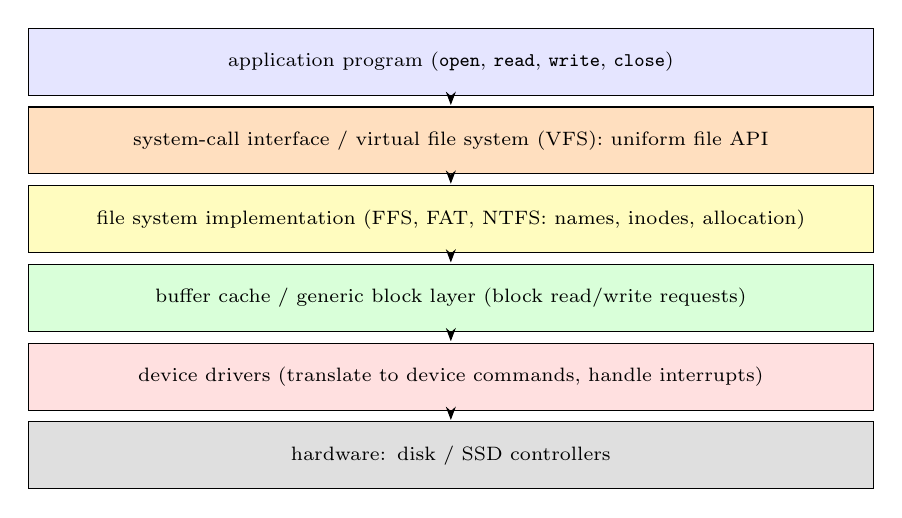
\begin{tikzpicture}[>=Stealth,font=\small]
\tikzstyle{b}=[draw,text width=10.5cm,minimum height=0.85cm,align=center,font=\scriptsize]
\node[b,fill=blue!10] at (0,0) {application program (\texttt{open}, \texttt{read}, \texttt{write}, \texttt{close})};
\node[b,fill=orange!25] at (0,-1.0) {system-call interface / virtual file system (VFS): uniform file API};
\node[b,fill=yellow!25] at (0,-2.0) {file system implementation (FFS, FAT, NTFS: names, inodes, allocation)};
\node[b,fill=green!15] at (0,-3.0) {buffer cache / generic block layer (block read/write requests)};
\node[b,fill=red!12] at (0,-4.0) {device drivers (translate to device commands, handle interrupts)};
\node[b,fill=gray!25] at (0,-5.0) {hardware: disk / SSD controllers};
\foreach \y in {-0.5,-1.5,-2.5,-3.5,-4.5} \draw[->] (0,\y+0.05) -- (0,\y-0.05);
\end{tikzpicture}
\end{document}
